% =============================================================================
//home/markov/Git/latex/0_includes/0_preamble.tex

%  {{{

\makeatletter
% \overarrow@ and \arrowfill@ are defined in amsmath
\newcommand*{\harpoon}{\mathpalette{\overarrow@\rightharpoonupfill@}}
\newcommand*{\rightharpoonupfill@}{\arrowfill@\relbar\relbar\rightharpoonup}
\makeatother

\DeclareFontFamily{U}{matha}{\hyphenchar\font45}
\DeclareFontShape{U}{matha}{m}{n}{
      <5> <6> <7> <8> <9> <10> gen * matha
      <10.95> matha10 <12> <14.4> <17.28> <20.74> <24.88> matha12
      }{}
\DeclareSymbolFont{matha}{U}{matha}{m}{n}
\DeclareMathSymbol{\varrightharpoonup}{3}{matha}{"E1}

% }}}

% ============================================================================ 
\begin{document}
%% Suppresses headers and footers on the title page
\begin{titlepage}

	% Centre everything on the title page
	\centering

	% Use small caps for all text on the title page
	\scshape

	% White space at the top of the page
	\vspace*{\baselineskip}

	%------------------------------------------------
	%	Title
	%------------------------------------------------

	% Thick horizontal rule
	\rule{\textwidth}{1.6pt}\vspace*{-\baselineskip}\vspace*{2pt}

	% Thin horizontal rule
	\rule{\textwidth}{0.4pt}

	% Whitespace above the title
	\vspace{0.75\baselineskip}

	% Title
	{\LARGE TITLE \\}

	% Whitespace below the title
	\vspace{0.75\baselineskip}

	% Thin horizontal rule
	\rule{\textwidth}{0.4pt}\vspace*{-\baselineskip}\vspace{3.2pt}

	% Thick horizontal rule
	\rule{\textwidth}{1.6pt}

	\vspace{2\baselineskip} % Whitespace after the title block

	%------------------------------------------------
	% Subtitle
	%------------------------------------------------

	% Kurt Wolff Verlag, Leipzig, 1927
	\vspace*{3\baselineskip} % Whitespace under the subtitle

	%------------------------------------------------
	% Author(s)
	%------------------------------------------------
	
%	Author
	by

	% Whitespace before the editors
	\vspace{0.5\baselineskip}

	% Author list
	{\scshape\Large John Doe  \\}

	\vspace*{3\baselineskip} % Whitespace under the subtitle

	%------------------------------------------------
	%	Editor(s)
	%------------------------------------------------
	
%	Edited By

	% Whitespace before the editors
%	\vspace{0.5\baselineskip}

	% Editor list
%	{\scshape\Large John Smith \\ Jane Smith \\}

	% Whitespace below the editor list
%	\vspace{0.5\baselineskip}

	% Editor affiliation
%	\textit{The University of California \\ Berkeley}

	% Whitespace between editor names and publisher logo
	\vfill

	%------------------------------------------------
	% Publisher
	%------------------------------------------------

	% Whitespace under the publisher logo
	\vspace{0.3\baselineskip}

	% Publisher
%	{\large TheVirtualLibrary.org} \\

	% Publication year
%	2019

	{\large Last Edited : } \today \\

\end{titlepage}

\raggedbottom
\twocolumn
%\onecolumn

\tableofcontents
\pagebreak

%\listoftables
%\vspace{1cm}
%\listoffigures
%\clearpage

%\onecolumn
\justifying 
\linenumbers




% SECTION : algebra {{{
\section{Algebra}
\label{sec:algebra}
\parindent=0em

\textbf{Logarithms}
\begin{itemize}[noitemsep]
	\item \( \log_{e}                              = \ln                                  \)
	\item \( \log_{a}{a}                           = 1                                    \)
	\item \( \log_{a}{(1)}                         = 0                                    \)
	\item \( \log_{a}{\left( \frac{1}{a} \right)}  = -1                                   \)
	\item \( \log_{a}{(n)} + \log_{a}{(m)}         = \log_{a}{(mn)}                       \)
	\item \( \log_{a}{(n)} - \log_{a}{(m)}         = \log_{a}{\left( \frac{m}{n} \right)} \)
	\item \( \log_{a}{(x^n)}                       = n \cdot \log_{a}{(x)}                \)
	\item \( \log_{a}{\left( \frac{1}{y} \right)}  = - \log_{a}{(y)}                      \)
\end{itemize}

\textbf{Exponentials}
\begin{itemize}[noitemsep]
	\item \( a^{m} \cdot a^{n} = a^{m+n}                                     \)
	\item \( a^{0}             = 1 \;\; (a \neq 0)                           \)
	\item \( a^{-n}            = \frac{1}{n}  \;\; (a \neq 0)                \)
	\item \( \frac{a^m}{a^n}   = a^{m-n} \;\; (a \neq 0)                     \)
	\item \( (a^m)^n = a^{mn}                                                \)
	\item \( (ab)^m = a^m b^m                                                \)
	\item \(  \left( \frac{a}{b} \right)^m = \frac{a^m}{b^m} \;\; (b \neq 0) \)
\end{itemize}




\textbf{Trigonometery} \\
\begin{tabular}{c|c|c|c|c|c|c|c|c|c}

deg
& \( 0^\circ   \)
& \( 30^\circ  \)
& \( 45^\circ  \)
& \( 60^\circ  \)
& \( 90^\circ  \)
& \( 180^\circ \)
& \( 270^\circ \)
& \( 360^\circ \)
\\ \midrule

rad
& \( 0              \)
& \( \frac{\pi}{6}  \)
& \( \frac{\pi}{4}  \)
& \( \frac{\pi}{3}  \)
& \( \frac{\pi}{2}  \)
& \( \pi            \)
& \( \frac{3\pi}{2} \)
& \( 2\pi           \)
\\ \midrule

\( \sin(\theta)         \)
& \( 0                  \)
& \( \frac{1}{2}        \)
& \( \frac{1}{\sqrt{2}} \)
& \( \frac{\sqrt{3}}{2} \)
& \( 1                  \)
& \( 0                  \)
& \( -1                 \)
& \( 0                  \)
\\ \midrule

\( \cos(\theta)         \)
& \( 1                  \)
& \( \frac{\sqrt{3}}{2} \)
& \( \frac{1}{\sqrt{2}} \)
& \( \frac{1}{2}        \)
& \( 0                  \)
& \( -1                 \)
& \( 0                  \)
& \( 1                  \)
\\ \midrule

\( \tan(\theta)         \)
& \( 0                  \)
& \( \frac{1}{\sqrt{3}} \)
& \( 1                  \)
& \( \sqrt{3}           \)
& \( N/A                \)
& \( 0                  \)
& \( N/A                \)
& \( 1                  \)
\\ \midrule

\end{tabular}




\sectionend
% }}} END SECTION : algebra


% SECTION : graphs {{{
\clearpage
\section{Graphs}
\label{sec:graphs}
\parindent=0em



% sin(x)  {{{

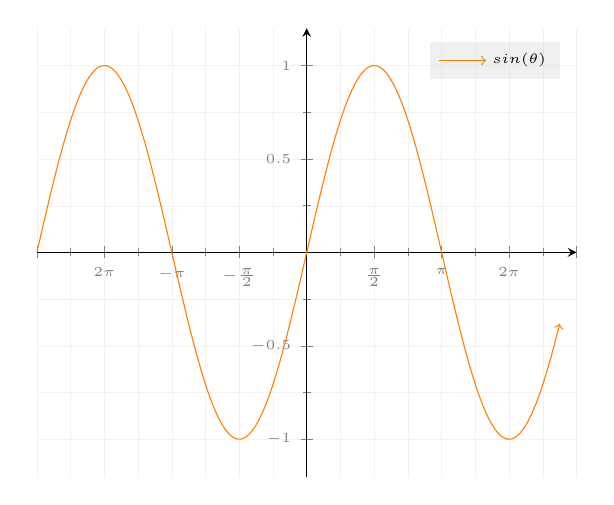
\begin{tikzpicture}
% axis settings {{{

\begin{axis}[
%	title          = graph_name,
	axis x line    = middle, % x-axis position
	axis y line    = middle, % y-axis position
	minor tick num = 1,      % num axis ticks
	grid           = both,
	grid style     =
	{
		line width = .1pt,
		draw       = gray!10
	},
	xmax      = 8,
	xmin      = -8,
	ymax      = 1.2,
	ymin      = -1.2,
	tick label style = {
		font  = \tiny,
		color = gray
	},
%	extra x ticks={3,1},
%	extra x tick labels={$\leftarrow$,$\rightarrow$},
%	extra y ticks={3,1},
%	extra y tick labels={$\leftarrow$,$\rightarrow$},
    xticklabels={ , , \( 2\pi \) , \( -\pi \) , \( -\frac{\pi}{2}  \) ,0, \( \frac{\pi}{2}  \), \( \pi \), \( 2\pi \)},
	legend style =
	{
		draw         = none, % remove legend bounding box
		font         = \tiny,
		legend pos   = north east,
		cells        = {anchor = west},
		fill         = gray!30,
		fill opacity = 0.4,
		text opacity = 1
	},
	%xlabel       = {$\scriptstyle rad$},
	%ylabel       = {$\scriptstyle y$},
	xlabel style =
	{
		at     = {(ticklabel* cs:1)},
%		anchor = north west
	},
	ylabel style =
	{
		at     = {(ticklabel* cs:1)},
%		anchor = south west
	}
]
% }}}
\coordinate (O) at (0,0);

\addplot [
	domain=-8:7.5,
	samples=300,
	orange,
	->
]
{sin(deg(\x*pi/4))};
\addlegendentry{$sin(\theta)$};


\end{axis}
\end{tikzpicture}

% }}}
% cos(x)  {{{

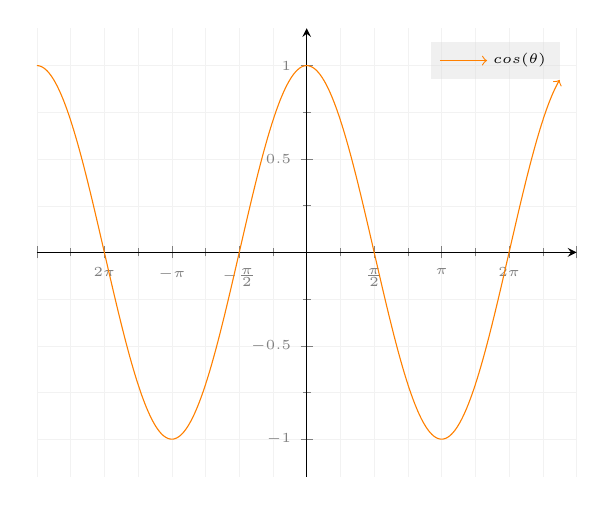
\begin{tikzpicture}
% axis settings {{{

\begin{axis}[
%	title          = graph_name,
	axis x line    = middle, % x-axis position
	axis y line    = middle, % y-axis position
	minor tick num = 1,      % num axis ticks
	grid           = both,
	grid style     =
	{
		line width = .1pt,
		draw       = gray!10
	},
	xmax      = 8,
	xmin      = -8,
	ymax      = 1.2,
	ymin      = -1.2,
	tick label style = {
		font  = \tiny,
		color = gray
	},
%	extra x ticks={3,1},
%	extra x tick labels={$\leftarrow$,$\rightarrow$},
%	extra y ticks={3,1},
%	extra y tick labels={$\leftarrow$,$\rightarrow$},
    xticklabels={ , , \( 2\pi \) , \( -\pi \) , \( -\frac{\pi}{2}  \) ,0, \( \frac{\pi}{2}  \), \( \pi \), \( 2\pi \)},
	legend style =
	{
		draw         = none, % remove legend bounding box
		font         = \tiny,
		legend pos   = north east,
		cells        = {anchor = west},
		fill         = gray!30,
		fill opacity = 0.4,
		text opacity = 1
	},
	%xlabel       = {$\scriptstyle rad$},
	%ylabel       = {$\scriptstyle y$},
	xlabel style =
	{
		at     = {(ticklabel* cs:1)},
%		anchor = north west
	},
	ylabel style =
	{
		at     = {(ticklabel* cs:1)},
%		anchor = south west
	}
]
% }}}
\coordinate (O) at (0,0);

\addplot [
	domain=-8:7.5,
	samples=300,
	orange,
	->
]
{cos(deg(\x*pi/4))};
\addlegendentry{$cos(\theta)$};


\end{axis}
\end{tikzpicture}

% }}}

% ln(x)  {{{

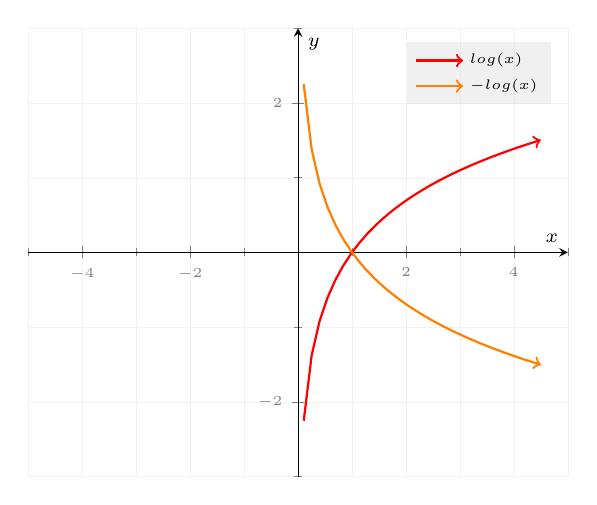
\begin{tikzpicture}
% axis settings {{{

\begin{axis}[
%	title          = graph_name,
	axis x line    = middle, % x-axis position
	axis y line    = middle, % y-axis position
	minor tick num = 1,      % num axis ticks
	grid           = both,
	grid style     =
	{
		line width = .1pt,
		draw       = gray!10
	},
	xmax      = 5,
	xmin      = -5,
	ymax      = 3,
	ymin      = -3,
	tick label style = {
		font  = \tiny,
		color = gray
	},
%	extra x ticks={3,1},
%	extra x tick labels={$\leftarrow$,$\rightarrow$},
%	extra y ticks={3,1},
%	extra y tick labels={$\leftarrow$,$\rightarrow$},
	legend style =
	{
		draw         = none, % remove legend bounding box
		font         = \tiny,
		legend pos   = north east,
		cells        = {anchor = west},
		fill         = gray!30,
		fill opacity = 0.4,
		text opacity = 1
	},
	xlabel       = {$\scriptstyle x$},
	ylabel       = {$\scriptstyle y$},
	xlabel style =
	{
		at     = {(ticklabel* cs:1)},
%		anchor = north west
	},
	ylabel style=
	{
		at     = {(ticklabel* cs:1)},
%		anchor = south west
	}
]
% }}}
\coordinate (O) at (0,0);

\addplot [
	domain=-10:4.5,
	samples=100,
	thick,
	red,
	->
]
{ln(x)};
\addlegendentry{$log(x)$};

\addplot [
	domain=-10:4.5,
	samples=100,
	thick,
	orange,
	->
]
{-ln(x)};
\addlegendentry{$-log(x)$};
\end{axis}
\end{tikzpicture}

% }}}
% ln(-x)  {{{

\begin{tikzpicture}
% axis settings {{{

\begin{axis}[
%	title          = graph_name,
	axis x line    = middle, % x-axis position
	axis y line    = middle, % y-axis position
	minor tick num = 1,      % num axis ticks
	grid           = none,
	grid style     =
	{
		line width = .1pt,
		draw       = gray!30
	},
	xmax      = 5,
	xmin      = -5,
	ymax      = 3,
	ymin      = -3,
	tick label style = {
		font  = \tiny,
		color = gray!30
	},
%	extra x ticks={3,1},
%	extra x tick labels={$\leftarrow$,$\rightarrow$},
%	extra y ticks={3,1},
%	extra y tick labels={$\leftarrow$,$\rightarrow$},
	legend style =
	{
		draw         = none, % remove legend bounding box
		font         = \tiny,
		legend pos   = outer north east,
		cells        = {anchor = west},
		fill         = gray,
		fill opacity = 0.4,
		text opacity = 1
	},
	xlabel       = {$\scriptstyle x$},
	ylabel       = {$\scriptstyle y$},
	xlabel style =
	{
		at     = {(ticklabel* cs:1)},
%		anchor = north west
	},
	ylabel style=
	{
		at     = {(ticklabel* cs:1)},
%		anchor = south west
	}
]
% }}}

\coordinate (O) at (0,0);

\addplot [
	domain=-10:10,
	samples=100,
	thick,
	orange,
	->
]
{ln(-x)};
%\addlegendentry{$\frac{1}{1+e^{-x}}$};

\end{axis}
\end{tikzpicture}

% }}}

% e^x  {{{

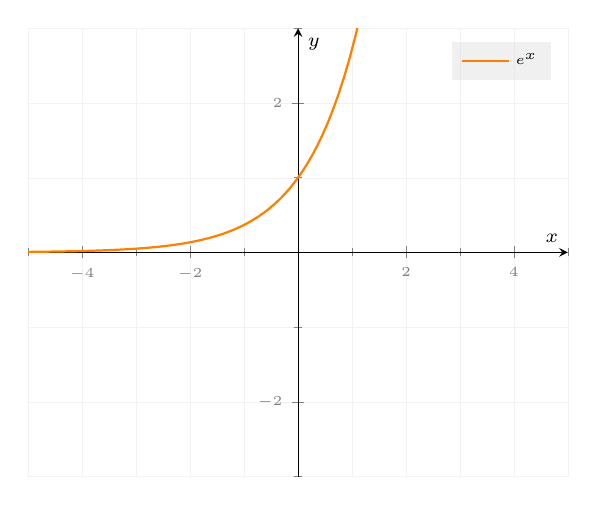
\begin{tikzpicture}
% axis settings {{{

\begin{axis}[
%	title          = graph_name,
	axis x line    = middle, % x-axis position
	axis y line    = middle, % y-axis position
	minor tick num = 1,      % num axis ticks
	grid           = both,
	grid style     =
	{
		line width = .1pt,
		draw       = gray!10
	},
	xmax      = 5,
	xmin      = -5,
	ymax      = 3,
	ymin      = -3,
	tick label style = {
		font  = \tiny,
		color = gray
	},
%	extra x ticks={3,1},
%	extra x tick labels={$\leftarrow$,$\rightarrow$},
%	extra y ticks={3,1},
%	extra y tick labels={$\leftarrow$,$\rightarrow$},
	legend style =
	{
		draw         = none, % remove legend bounding box
		font         = \tiny,
		legend pos   = north east,
		cells        = {anchor = west},
		fill         = gray!30,
		fill opacity = 0.4,
		text opacity = 1
	},
	xlabel       = {$\scriptstyle x$},
	ylabel       = {$\scriptstyle y$},
	xlabel style =
	{
		at     = {(ticklabel* cs:1)},
%		anchor = north west
	},
	ylabel style=
	{
		at     = {(ticklabel* cs:1)},
%		anchor = south west
	}
]
% }}}
\coordinate (O) at (0,0);

\addplot [
	domain=-5:5,
	no marks,
	samples=100,
	thick,
	orange
]
{exp(x)};
\addlegendentry{$e^x$};

\end{axis}
\end{tikzpicture}

% }}}
% sqrt(x)  {{{

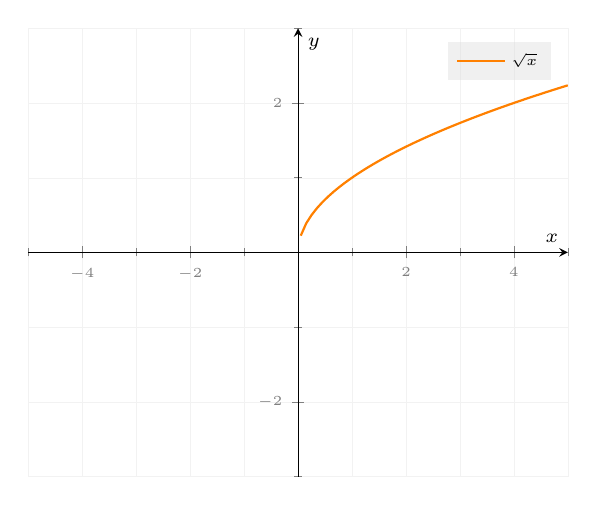
\begin{tikzpicture}
% axis settings {{{

\begin{axis}[
%	title          = graph_name,
	axis x line    = middle, % x-axis position
	axis y line    = middle, % y-axis position
	minor tick num = 1,      % num axis ticks
	grid           = both,
	grid style     =
	{
		line width = .1pt,
		draw       = gray!10
	},
	xmax      = 5,
	xmin      = -5,
	ymax      = 3,
	ymin      = -3,
	tick label style = {
		font  = \tiny,
		color = gray
	},
%	extra x ticks={3,1},
%	extra x tick labels={$\leftarrow$,$\rightarrow$},
%	extra y ticks={3,1},
%	extra y tick labels={$\leftarrow$,$\rightarrow$},
	legend style =
	{
		draw         = none, % remove legend bounding box
		font         = \tiny,
		legend pos   = north east,
		cells        = {anchor = west},
		fill         = gray!30,
		fill opacity = 0.4,
		text opacity = 1
	},
	xlabel       = {$\scriptstyle x$},
	ylabel       = {$\scriptstyle y$},
	xlabel style =
	{
		at     = {(ticklabel* cs:1)},
%		anchor = north west
	},
	ylabel style=
	{
		at     = {(ticklabel* cs:1)},
%		anchor = south west
	}
]
% }}}
\coordinate (O) at (0,0);

\addplot [
	domain=-5:5,
	no marks,
	samples=100,
	thick,
	orange
]
{sqrt(x)};
\addlegendentry{$\sqrt{x}$};


\end{axis}
\end{tikzpicture}

% }}}


% y=x^(-1)  {{{
\begin{tikzpicture}
% axis settings {{{

\begin{axis}[
%	title          = graph_name,
	axis x line    = middle, % x-axis position
	axis y line    = middle, % y-axis position
	minor tick num = 1,      % num axis ticks
	grid           = none,
	grid style     =
	{
		line width=.1pt,
		draw=gray!30
	},
	xmax = 5,
	xmin = -5,
	ymax = 10,
	ymin = -10,
	tick label style = {
		font = \tiny,
		color = white
	},
%	extra x ticks={3,1},
%	extra x tick labels={$\leftarrow$,$\rightarrow$},
%	extra y ticks={3,1},
%	extra y tick labels={$\leftarrow$,$\rightarrow$},
	legend style =
	{
		draw         = none, % remove legend bounding box
		font         = \tiny,
		legend pos   = outer north east,
		cells        = {anchor = west},
		fill         = gray,
		fill opacity = 0.4,
		text opacity = 1
	},
	xlabel       = {$\scriptstyle x$},
	ylabel       = {$\scriptstyle y$},
	xlabel style =
	{
		at     = {(ticklabel* cs:1)},
%		anchor = north west
	},
	ylabel style=
	{
		at     = {(ticklabel* cs:1)},
%		anchor = south west
	}
]
% }}}

\coordinate (O) at (0,0);

\addplot [
	domain=-5:5,
	no marks,
	samples=100,
	thick,
	orange
]
{x^(-1)};
%\addlegendentry{$\frac{1}{1+e^{-x}}$};

\end{axis}
\end{tikzpicture}

% }}}
% y=x^2  {{{
\begin{tikzpicture}
% axis settings {{{

\begin{axis}[
%	title          = graph_name,
	axis x line    = middle, % x-axis position
	axis y line    = middle, % y-axis position
	minor tick num = 1,      % num axis ticks
	grid           = none,
	grid style     =
	{
		line width=.1pt,
		draw=gray!30
	},
	xmax = 5,
	xmin = -5,
	ymax = 10,
	ymin = -10,
	tick label style = {
		font = \tiny,
		color = white
	},
%	extra x ticks={3,1},
%	extra x tick labels={$\leftarrow$,$\rightarrow$},
%	extra y ticks={3,1},
%	extra y tick labels={$\leftarrow$,$\rightarrow$},
	legend style =
	{
		draw         = none, % remove legend bounding box
		font         = \tiny,
		legend pos   = outer north east,
		cells        = {anchor = west},
		fill         = gray,
		fill opacity = 0.4,
		text opacity = 1
	},
	xlabel       = {$\scriptstyle x$},
	ylabel       = {$\scriptstyle y$},
	xlabel style =
	{
		at     = {(ticklabel* cs:1)},
%		anchor = north west
	},
	ylabel style=
	{
		at     = {(ticklabel* cs:1)},
%		anchor = south west
	}
]
% }}}

\coordinate (O) at (0,0);

\addplot [
	domain=-5:5,
	no marks,
	samples=100,
	thick,
	orange
]
{x^2};
%\addlegendentry{$\frac{1}{1+e^{-x}}$};

\end{axis}
\end{tikzpicture}

% }}}
% y=x^(1/2)  {{{
\begin{tikzpicture}
% axis settings {{{

\begin{axis}[
%	title          = graph_name,
	axis x line    = middle, % x-axis position
	axis y line    = middle, % y-axis position
	minor tick num = 1,      % num axis ticks
	grid           = none,
	grid style     =
	{
		line width=.1pt,
		draw=gray!30
	},
	xmax = 5,
	xmin = -5,
	ymax = 3,
	ymin = -3,
	tick label style = {
		font = \tiny,
		color = white
	},
%	extra x ticks={3,1},
%	extra x tick labels={$\leftarrow$,$\rightarrow$},
%	extra y ticks={3,1},
%	extra y tick labels={$\leftarrow$,$\rightarrow$},
	legend style =
	{
		draw         = none, % remove legend bounding box
		font         = \tiny,
		legend pos   = outer north east,
		cells        = {anchor = west},
		fill         = gray,
		fill opacity = 0.4,
		text opacity = 1
	},
	xlabel       = {$\scriptstyle x$},
	ylabel       = {$\scriptstyle y$},
	xlabel style =
	{
		at     = {(ticklabel* cs:1)},
%		anchor = north west
	},
	ylabel style=
	{
		at     = {(ticklabel* cs:1)},
%		anchor = south west
	}
]
% }}}

\coordinate (O) at (0,0);

\addplot [
	domain=-5:5,
	no marks,
	samples=100,
	thick,
	orange
]
{x^(1/2)};
%\addlegendentry{$\frac{1}{1+e^{-x}}$};

\end{axis}
\end{tikzpicture}

% }}}
% y=x^3  {{{
\begin{tikzpicture}
% axis settings {{{

\begin{axis}[
%	title          = graph_name,
	axis x line    = middle, % x-axis position
	axis y line    = middle, % y-axis position
	minor tick num = 1,      % num axis ticks
	grid           = none,
	grid style     =
	{
		line width=.1pt,
		draw=gray!30
	},
	xmax = 5,
	xmin = -5,
	ymax = 10,
	ymin = -10,
	tick label style = {
		font = \tiny,
		color = white
	},
%	extra x ticks={3,1},
%	extra x tick labels={$\leftarrow$,$\rightarrow$},
%	extra y ticks={3,1},
%	extra y tick labels={$\leftarrow$,$\rightarrow$},
	legend style =
	{
		draw         = none, % remove legend bounding box
		font         = \tiny,
		legend pos   = outer north east,
		cells        = {anchor = west},
		fill         = gray,
		fill opacity = 0.4,
		text opacity = 1
	},
	xlabel       = {$\scriptstyle x$},
	ylabel       = {$\scriptstyle y$},
	xlabel style =
	{
		at     = {(ticklabel* cs:1)},
%		anchor = north west
	},
	ylabel style=
	{
		at     = {(ticklabel* cs:1)},
%		anchor = south west
	}
]
% }}}

\coordinate (O) at (0,0);

\addplot [
	domain=-5:5,
	no marks,
	samples=100,
	thick,
	orange
]
{x^3};
%\addlegendentry{$\frac{1}{1+e^{-x}}$};

\end{axis}
\end{tikzpicture}

% }}}

% y=2^x  {{{
\begin{tikzpicture}
% axis settings {{{

\begin{axis}[
%	title          = graph_name,
	axis x line    = middle, % x-axis position
	axis y line    = middle, % y-axis position
	minor tick num = 1,      % num axis ticks
	grid           = none,
	grid style     =
	{
		line width=.1pt,
		draw=gray!30
	},
	xmax = 5,
	xmin = -5,
	ymax = 10,
	ymin = -10,
	tick label style = {
		font = \tiny,
		color = white
	},
%	extra x ticks={3,1},
%	extra x tick labels={$\leftarrow$,$\rightarrow$},
%	extra y ticks={3,1},
%	extra y tick labels={$\leftarrow$,$\rightarrow$},
	legend style =
	{
		draw         = none, % remove legend bounding box
		font         = \tiny,
		legend pos   = outer north east,
		cells        = {anchor = west},
		fill         = gray,
		fill opacity = 0.4,
		text opacity = 1
	},
	xlabel       = {$\scriptstyle x$},
	ylabel       = {$\scriptstyle y$},
	xlabel style =
	{
		at     = {(ticklabel* cs:1)},
%		anchor = north west
	},
	ylabel style=
	{
		at     = {(ticklabel* cs:1)},
%		anchor = south west
	}
]
% }}}

\coordinate (O) at (0,0);

\addplot [
	domain=-5:5,
	no marks,
	samples=100,
	thick,
	orange
]
{2^(x)};
%\addlegendentry{$\frac{1}{1+e^{-x}}$};

\end{axis}
\end{tikzpicture}

% }}}
% y=abs(x)  {{{
\begin{tikzpicture}
% axis settings {{{

\begin{axis}[
%	title          = graph_name,
	axis x line    = middle, % x-axis position
	axis y line    = middle, % y-axis position
	minor tick num = 1,      % num axis ticks
	grid           = none,
	grid style     =
	{
		line width=.1pt,
		draw=gray!30
	},
	xmax = 5,
	xmin = -5,
	ymax = 10,
	ymin = -10,
	tick label style = {
		font = \tiny,
		color = white
	},
%	extra x ticks={3,1},
%	extra x tick labels={$\leftarrow$,$\rightarrow$},
%	extra y ticks={3,1},
%	extra y tick labels={$\leftarrow$,$\rightarrow$},
	legend style =
	{
		draw         = none, % remove legend bounding box
		font         = \tiny,
		legend pos   = outer north east,
		cells        = {anchor = west},
		fill         = gray,
		fill opacity = 0.4,
		text opacity = 1
	},
	xlabel       = {$\scriptstyle x$},
	ylabel       = {$\scriptstyle y$},
	xlabel style =
	{
		at     = {(ticklabel* cs:1)},
%		anchor = north west
	},
	ylabel style=
	{
		at     = {(ticklabel* cs:1)},
%		anchor = south west
	}
]
% }}}

\coordinate (O) at (0,0);

\addplot [
	domain=-5:5,
	no marks,
	samples=100,
	thick,
	orange
]
{abs(x)};
%\addlegendentry{$\frac{1}{1+e^{-x}}$};

\end{axis}
\end{tikzpicture}

% }}}


% sigmoid  {{{

\begin{tikzpicture}
% axis settings {{{

\begin{axis}[
%	title          = graph_name,
	axis x line    = middle, % x-axis position
	axis y line    = middle, % y-axis position
	minor tick num = 1,      % num axis ticks
	grid           = none,
	grid style     =
	{
		line width=.1pt,
		draw=gray!30
	},
	xmax = 10,
	xmin = -10,
	ymax = 1.05, % 0.05 is to show the ->
	ymin = -1.05,
	tick label style = {
		font = \tiny,
		color = white
	},
%	extra x ticks={3,1},
%	extra x tick labels={$\leftarrow$,$\rightarrow$},
%	extra y ticks={3,1},
%	extra y tick labels={$\leftarrow$,$\rightarrow$},
	legend style =
	{
		draw         = none, % remove legend bounding box
		font         = \tiny,
		legend pos   = outer north east,
		cells        = {anchor = west},
		fill         = gray,
		fill opacity = 0.4,
		text opacity = 1
	},
	xlabel       = {$\scriptstyle x$},
	ylabel       = {$\scriptstyle y$},
	xlabel style =
	{
		at     = {(ticklabel* cs:1)},
%		anchor = north west
	},
	ylabel style=
	{
		at     = {(ticklabel* cs:1)},
%		anchor = south west
	}
]
% }}}

\coordinate (O) at (0,0);

\addplot [
	domain=-10:10,
	no marks,
	samples=100,
	thick,
	orange,
	->
]
{1/(1+exp(-x)};
%\addlegendentry{$\frac{1}{1+e^{-x}}$};

\end{axis}
\end{tikzpicture}

% }}}

% hyperbolic_tangent
% cube root x


\pagebreak






\sectionend
% }}} END SECTION : graphs



% SECTION : linear_algebra {{{
\section{Linear Algebra}
\label{sec:linear_algebra}
\parindent=0em

% 	SUB-SECTION : basics {{{
\subsection{Basics}
\label{ssec:basics}
\parindent=0em

\[
	\begin{aligned}
		\harpoon{a} + \harpoon{b} & = \harpoon{b} + \harpoon{a} \\
		2\harpoon{a}              & = \harpoon{a} + \harpoon{a} \\
		{\|\harpoon{a}\|}^{2}     & = \sum_{i}{a}_{i}^{2} \\
		A^{T}_{ij}                & = A_{ji}
	\end{aligned}
\]

% 		SUB-SUB-SECTION : matrix_multiplication {{{
\subsubsection{Matrix Multiplication}
\label{sssec:matrix_multiplication}
\parindent=0em

\textbf {Right way to think about it}


\subsubsectionend
% }}} END SUB-SUB-SECTION : matrix_multiplication

\textbf{Why is it called Linear Algebra ?}

\textbf {Linear Transformations}

\subsectionend
% }}} END SUB-SECTION : basics

% 	SUB-SECTION : basis {{{
\subsection{Basis}
\label{ssec:basis}
\parindent=0em

% DEFINITION : basis_vector {{{
\tcolorboxdefinition
{Basis Vector}
{\label{def:basis_vector}}
{

The set of vectors that are used to define the co-ordinate system that we are
operating in , are called basis vectors.

}

% }}} END DEFINITION : basis_vector

Every time that we define two vectors , we are also simultaneously making a choice for what basis we are operating in. It just so happends that most often , this basis is on the x , y plane with \( \hat{i} \) , and \( \hat{j} \) being the basis vectors.

% DEFINITION : span {{{
\tcolorboxdefinition
{Span}
{\label{def:span}}
{

All the points that you can reach in a plane with the basis vectors that you chose is called the span.

The span of \( \harpoon{a} \) and \( \harpoon{b} \) is the set of all of their linear combinations , i.e. , \( x \harpoon{a} + y \harpoon{b} , \text{where} \; x,y \in \mathbb{R} \).

}

Usually most basis vectors will you give you the entire plane , except if they line up , i.e, if the angle between them is 0 , or if both vectors are just 0.

A vector is called \textbf {linearly dependent} on another if it is in the span of the other. If a vector adds another dimension then it is \textbf{linearly independent}.

The scalar projection of your basis vector onto another is how you find out what the scalar value of that vector is , in the span defined by your chosen basis vector.

Basically , \( \harpoon{v} \) in basis  \( \harpoon{b_1} \) , \( \harpoon{b_2} \) , where \( \harpoon{b_1} \) , \( \harpoon{b_2} \) are orthogonal to each other , is given by 

\[
\begin{aligned}
\begin{bmatrix}
\frac{\harpoon{v} \bullet \harpoon{b_1}}{\left\|\harpoon{b_1}\right\|} \\
\frac{\harpoon{v} \bullet \harpoon{b_2}}{\left\|\harpoon{b_2}\right\|}
\end{bmatrix}
\end{aligned}
\]


% }}} END DEFINITION : span

Maps of images in CNNs can be thought of as basis changes and vector projections to more feature rich spaces.


% 		SUB-SUB-SECTION : converting_basis {{{
\subsubsection{Converting Basis}
\label{sssec:converting_basis}
\parindent=0em

%If the basis vectors are orthogonal ( \( 90^\circ \) ) , you can just use projections to calculate what the vector in the new basis would be.

%Else you have to find a matrix \( A \) to transform vector \( \harpoon{r} \) from basis \( b_1 \) , such that \( A \harpoon{r}_{b_1} \) gives me the vector \( \harpoon{r_{b_2}}\) in the new basis \( b_2 \). Similarly \( A^{-1}\harpoon{r_{b_2}} \) gives me the vector \( \harpoon{r} \) back in basis \( b_1 \).

%This matrix \( A \) is built by :
%Here we are converting from first basis \( b_1 \) , to new basis \( b_2 \). The basis vectors for \( b_2 \) are \( b_2_{x} , b_2_{y} \).
%\[
  %A =
	%\left[
		%{
		%\begin{array}{cc}
			%b_2_{x} & b_2_{y} \\
		%\end{array}
		%}
	%\right]
	%=
	%\left[
		%{
		%\begin{array}{cc}
			%b_2_{x_1} & b_2_{y_1} \\
			%b_2_{x_2} & b_2_{y_2} \\
		%\end{array}
		%}
	%\right]
%\]

%and accordingly \( A^{-1} \) is :

%\[
	%A^{-1} =
	%\frac{1}{ad-bc}
	%\left[
		%{
		%\begin{array}{cc}
			%d  & -b \\
			%-c & a \\
		%\end{array}
		%}
	%\right]
%\]

\subsubsectionend
% }}} END SUB-SUB-SECTION : converting_basis

% 		SUB-SUB-SECTION : rotating_in_a_different_basis {{{
\subsubsection{Rotating in a different Basis}
\label{sssec:rotating_in_a_different_basis}
\parindent=0em

Figure out matrix \( A \) that transforms from basis \( b_1 \) to \( b_2 \).

Figure out the rotation as a transformation by matrix multiplication in basis \( b_1 \) , i.e. find the matrix that you need to multiply by for that rotation.

Transform the vector that the transformation needs to be applied to , from basis \( b_2 \) into basis \( b_1 \).

Apply the rotation by matrix multiplication in basis \( b_1 \).

Transformed the rotated matrix back into basis \( b_2 \) by multiplying by \( A^{-1} \).



\subsubsectionend
% }}} END SUB-SUB-SECTION : rotating_in_a_different_basis

\subsectionend
% }}} END SUB-SECTION : basis

% 	SUB-SECTION : products {{{
\subsection{Products}
\label{ssec:products}
\parindent=0em

% 		SUB-SUB-SECTION : inner_product {{{
\subsubsection{Inner Product}
\label{sssec:inner_product}
\parindent=0em

\[
	\begin{aligned}
		\harpoon{a} \bullet \harpoon{b}                         & = a_{1}b_{1}+a_{2}b_{2} + \ldots + a_{n}b_{n} \\
		                                                        & = \sum_{i}{a_{i}b_{i}} \\
	\harpoon{a} \bullet \harpoon{a}                             & = \left\| \harpoon{a} \right\|^{2} \\
	\harpoon{a} \bullet \harpoon{b}                             & = \harpoon{b} \bullet \harpoon{a} \\
	\harpoon{a} \bullet \left(\harpoon{b} + \harpoon{c} \right) & = \harpoon{a} \bullet \harpoon{b} + \harpoon{a} \bullet \harpoon{c} \\
	\harpoon{a} \bullet \left( x \harpoon{b} \right)            & = x \left(\harpoon{a} \bullet \harpoon{b}\right) \\
	\harpoon{a} \bullet \harpoon{b}                       & = \harpoon{a}\harpoon{b}^{T}
	\end{aligned}
\]



\subsubsectionend
% }}} END SUB-SUB-SECTION : inner_product
% 		SUB-SUB-SECTION : outer_product {{{
\subsubsection{Outer Product}
\label{sssec:outer_product}
\parindent=0em



\subsubsectionend
% }}} END SUB-SUB-SECTION : outer_product

\subsectionend
% }}} END SUB-SECTION : products

% 	SUB-SECTION : operations {{{
\subsection{Operations}
\label{ssec:operations}
\parindent=0em

% 		SUB-SUB-SECTION : projections {{{
\subsubsection{Projections}
\label{sssec:projections}
\parindent=0em

% projections  {{{


\begin{tikzpicture}
% axis settings {{{

\begin{axis}[
%	title          = graph_name,
	axis line style={white},
	axis x line    = middle, % x-axis position
	axis y line    = middle, % y-axis position
	minor tick num = 0,      % num axis ticks
	grid           = both,
	grid style     =
	{
		line width = .1pt,
		draw       = gray!10
	},
	xmax      = 6,
	xmin      = -3,
	ymax      = 6,
	ymin      = -3,
	tick label style = {
		font  = \tiny,
		color = white
	},
	ticks = none,
%	extra x ticks={3,1},
%	extra x tick labels={$\leftarrow$,$\rightarrow$},
%	extra y ticks={3,1},
%	extra y tick labels={$\leftarrow$,$\rightarrow$},
	legend style =
	{
		draw         = none, % remove legend bounding box
		font         = \tiny,
		legend pos   = north east,
		cells        = {anchor = west},
		fill         = gray!30,
		fill opacity = 0.4,
		text opacity = 1
	},
	%xlabel       = {$\scriptstyle rad$},
	%ylabel       = {$\scriptstyle y$},
	xlabel style =
	{
		at     = {(ticklabel* cs:1)},
%		anchor = north west
	},
	ylabel style =
	{
		at     = {(ticklabel* cs:1)},
%		anchor = south west
	}
]
% }}}

\coordinate (O) at (0,0);
\coordinate (v1) at (2,4);
\coordinate (v2) at (5,0);
\coordinate (proj) at (2,0);


\draw[thick,-Stealth] (O) -- (v1) node[above] { \( \vec{v} \) };
\draw[thick,-Stealth] (O) -- (v2) node[above] { \( \vec{w} \) };

\draw[dotted,-] (v1) -- (proj);
%\draw[thick,orange,-Stealth] (O) -- (proj);
\draw [
		decorate,
		pen colour={black},
		decoration = {
			calligraphic brace,
			amplitude = 5pt,
			mirror,
			raise = 5pt
		}
	]
	(O) -- (proj)
	node[pos=0.25,below=8pt,black]
	{ Proj. of}
	node[pos=0.25,below=20pt,black]
	{ \( \vec{v} \) onto \( \vec{w} \)};

	\draw pic[
		"$\theta$",
		draw=black,
		thick,
		-,
		angle eccentricity=1.5,
		angle radius=0.5cm
		]
	% start , mid , end
	{angle = v2--O--v1};

	%\draw pic[
		%draw=black,
		%-,
		%angle eccentricity=1.5,
		%angle radius=0.5cm
		%]
	%% start , mid , end
	%{angle = v1--proj--O};


\addplot [name path = A, -, domain = 0:2, samples = 100] {2*x};
\addplot [name path = B, -, domain = 0:2] {0};
\draw [thick] (-1,-3) +(-.4,0) |- +(0,.4);
\addplot [gray!30] fill between [of = A and B, soft clip={domain=0:2}];
 
%\draw[thick,orange,-Stealth] (O) -- (1,0) node[pos=-0.25,left] { \( \hat{w} = \frac{\vec{w}}{||\vec{w}||}  \) };

\end{axis}
\end{tikzpicture}

% }}}

\textbf{Scalar Projection}

It is the length (scalar) of the 'shadow' cast by one vector onto another.\\

It is basically how much \( \harpoon{a} \) goes in direction of \( \harpoon{b} \) as a scalar.

\[
\begin{aligned}
	\frac{\harpoon{a} \bullet \harpoon{b}}{\left\|\harpoon{a}\right\|} & = \left\|\harpoon{b}\right\| \; cos(\theta)
\end{aligned}
\]

\textbf{Vector Projection}

It is the a vector of the scalar projection , i.e. , how much \( \harpoon{a} \) goes in direction of \( \harpoon{b} \) , created by multiplying the scalar projection with a unit vector in direction of \( \harpoon{b} \).

Vector in direction \( \harpoon{a} \) with length 1 :
\[
	\frac{\harpoon{a}}{\left\| \harpoon{a} \right\|} 
\]

Vector Projection :

\[
\begin{aligned}
	\frac{\harpoon{a}}{\left\| \harpoon{a} \right\|} \; \frac{\harpoon{a} \bullet \harpoon{b}}{\left\|\harpoon{a}\right\|} 
	& = \harpoon{a} \; \frac{\harpoon{a} \bullet \harpoon{b}}{\harpoon{a} \bullet \harpoon{a}} \\
\end{aligned}
\]





\subsubsectionend
% }}} END SUB-SUB-SECTION : projections
% 		SUB-SUB-SECTION : rotations {{{
\subsubsection{Rotations}
\label{sssec:rotations}
\parindent=0em



\subsubsectionend
% }}} END SUB-SUB-SECTION : rotations
% 		SUB-SUB-SECTION : scale {{{
\subsubsection{Scale}
\label{sssec:scale}
\parindent=0em



\subsubsectionend
% }}} END SUB-SUB-SECTION : scale
% 		SUB-SUB-SECTION : shear {{{
\subsubsection{Shear}
\label{sssec:shear}
\parindent=0em



\subsubsectionend
% }}} END SUB-SUB-SECTION : shear
% 		SUB-SUB-SECTION : pivots {{{
\subsubsection{Pivots}
\label{sssec:pivots}
\parindent=0em



\subsubsectionend
% }}} END SUB-SUB-SECTION : pivots
% 		SUB-SUB-SECTION : transpose {{{
\subsubsection{Transpose}
\label{sssec:transpose}
\parindent=0em



\subsubsectionend
% }}} END SUB-SUB-SECTION : transpose
% 		SUB-SUB-SECTION : conjugate {{{
\subsubsection{Conjugate}
\label{sssec:conjugate}
\parindent=0em



\subsubsectionend
% }}} END SUB-SUB-SECTION : conjugate
% 		SUB-SUB-SECTION : complex_conjugate {{{
\subsubsection{Complex Conjugate}
\label{sssec:complex_conjugate}
\parindent=0em



\subsubsectionend
% }}} END SUB-SUB-SECTION : complex_conjugate

\subsectionend
% }}} END SUB-SECTION : operations

% 	SUB-SECTION : properties {{{
\subsection{Properties}
\label{ssec:properties}
\parindent=0em

Zero Matrix
Row Matrix
Column Matrix
Square Matrix
Diagonal Matrix
Symmetrix Matrix
Scalar Matrix
Null Matrix
Singular Matrix
Invertible Matrix
Transpose
Permutation Matrix
Orthogonal
Upper Triangular
Lower Triangular
Positive Definite Matrix
Positive Semi-Definite Matrix
Bilinearity
Ciculant Matrix
Orthogonal Matrix
Eigenvalue Matrix

% 		SUB-SUB-SECTION : orthogonoal {{{
\subsubsection{Orthogonoal}
\label{sssec:orthogonoal}
\parindent=0em

Orthogonal Matrices are a special kind of matrix that combine both inverse matrices and transpose matrices. Specifically they combine them in a way , such that for any matrix \( Q \) if \( Q^{-1} = Q^{T} \) , then \( Q \) is an Orthogonal Matrix. It is more commonly written as the following :

\[
	QQ^{T} = I = Q^{T}Q
\]

Properties :

\begin{itemize}[noitemsep]

	\item Orthogonal Matrix preservs norms / lengths : \(
		(Q \vec{x})^{T}(Q\vec{x}) = ||Q\vec{x}||^{2} = \vec{x}^{T}Q^{T}Q\vec{x} = \vec{x}^T\vec{x} = ||\vec{x}||^{2}
		\)

\end{itemize}


\textbf{Orthonormal}


\subsubsectionend
% }}} END SUB-SUB-SECTION : orthogonoal
% 		SUB-SUB-SECTION : positive {{{
\subsubsection{Positive}
\label{sssec:positive}
\parindent=0em



\subsubsectionend
% }}} END SUB-SUB-SECTION : positive

\subsectionend
% }}} END SUB-SECTION : properties

% 	SUB-SECTION : spaces {{{
\subsection{Spaces}
\label{ssec:spaces}
\parindent=0em

\textbf{Vector Spaces} \\
\textbf {Null Space} \\
\textbf {Column Space} \\
\textbf {Row Space} \\
\textbf {Eigenspace} \\
\textbf {Fundamental Theorem of Linear Algebra} \\

\subsectionend
% }}} END SUB-SECTION : spaces

% 	SUB-SECTION : eigenvectors {{{
\subsection{Eigenvectors}
\label{ssec:eigenvectors}
\parindent=0em

All vectors that stay on thier span post a transformation.


% projections  {{{


\begin{tikzpicture}
% axis settings {{{

\begin{axis}[
%	title          = graph_name,
	axis line style={white},
	axis x line    = middle, % x-axis position
	axis y line    = middle, % y-axis position
	minor tick num = 0,      % num axis ticks
	grid           = none,
	grid style     =
	{
		line width = .1pt,
		draw       = gray!10
	},
	xmax      = 6,
	xmin      = -2,
	ymax      = 6,
	ymin      = -2,
	ticks = none,
	%tick label style = {
		%font  = \tiny,
		%color = white
	%},
%	extra x ticks={3,1},
%	extra x tick labels={$\leftarrow$,$\rightarrow$},
%	extra y ticks={3,1},
%	extra y tick labels={$\leftarrow$,$\rightarrow$},
	legend style =
	{
		draw         = none, % remove legend bounding box
		font         = \tiny,
		legend pos   = north east,
		cells        = {anchor = west},
		fill         = gray!30,
		fill opacity = 0.4,
		text opacity = 1
	},
	%xlabel       = {$\scriptstyle rad$},
	%ylabel       = {$\scriptstyle y$},
	xlabel style =
	{
		at     = {(ticklabel* cs:1)},
%		anchor = north west
	},
	ylabel style =
	{
		at     = {(ticklabel* cs:1)},
%		anchor = south west
	}
]
% }}}

\coordinate (O) at (0,0);
\coordinate (A) at (0,2);
\coordinate (B) at (2,0);

\coordinate (X) at (0,10);
\coordinate (Y) at (10,0);

\draw [fill=black] (A) circle (1pt);
\draw [fill=black] (B) circle (1pt);

\draw[thin,-Stealth] (O) -- (A) node[above] { \( \vec{v} \) };
\draw[thin,-Stealth] (O) -- (B) node[above] { \( \vec{w} \) };

\draw[dashed,gray,-] (-10,0) -- (10,0);
\draw[dashed,gray,-] (0,-10) -- (0,10);


\end{axis}
\end{tikzpicture}

% }}}

\[
	\overrightarrow{transformation}
\]

% projections  {{{


\begin{tikzpicture}
% axis settings {{{

\begin{axis}[
%	title          = graph_name,
	axis line style={white},
	axis x line    = middle, % x-axis position
	axis y line    = middle, % y-axis position
	minor tick num = 0,      % num axis ticks
	grid           = none,
	grid style     =
	{
		line width = .1pt,
		draw       = gray!10
	},
	xmax      = 6,
	xmin      = -2,
	ymax      = 6,
	ymin      = -2,
	ticks = none,
	%tick label style = {
		%font  = \tiny,
		%color = white
	%},
%	extra x ticks={3,1},
%	extra x tick labels={$\leftarrow$,$\rightarrow$},
%	extra y ticks={3,1},
%	extra y tick labels={$\leftarrow$,$\rightarrow$},
	legend style =
	{
		draw         = none, % remove legend bounding box
		font         = \tiny,
		legend pos   = north east,
		cells        = {anchor = west},
		fill         = gray!30,
		fill opacity = 0.4,
		text opacity = 1
	},
	%xlabel       = {$\scriptstyle rad$},
	%ylabel       = {$\scriptstyle y$},
	xlabel style =
	{
		at     = {(ticklabel* cs:1)},
%		anchor = north west
	},
	ylabel style =
	{
		at     = {(ticklabel* cs:1)},
%		anchor = south west
	}
]
% }}}

\coordinate (O) at (0,0);
\coordinate (A) at (0,2);
\coordinate (B) at (2,0);

\coordinate (X) at (0,10);
\coordinate (Y) at (10,0);

%\draw [fill=black] (A) circle (1pt);
%\draw [fill=black] (B) circle (1pt);

%\draw[thin,-Stealth] (O) -- (A) node[above] { \( \vec{v} \) };
%\draw[thin,-Stealth] (O) -- (B) node[above] { \( \vec{w} \) };
\draw[thin,-Stealth] (O) -- (2,4) node[above] { \( T(\vec{v}) \) };
\draw[thin,-Stealth] (O) -- (4,0) node[above] { \( T(\vec{w}) \) };

\draw[dashed,gray,-] (-10,0) -- (10,0);
\draw[dashed,gray,-] (0,-10) -- (0,10);


\end{axis}
\end{tikzpicture}

% }}}

After the above transformation we can see that \( \vec{v} \) is an eigenvector of the transformation \( T \) , because it stays on its span (dotted line). Usually we scale the eigenvectors down to unit size by dividing by the magnitude \( \frac{\vec{v}}{||\vec{v}||}  \).


So for any transformation \( T(\vec(x)) \) in linear algebra , we can get a good picture of what \( T(\vec(x)) \) has done to our original space by just looking at the eigenvalues.

\[
	T \vec{x} = \lambda \vec{x}
\]

Where \( T \) is some transformation matrix , \( \lambda \) is the eigenvalue and \( \vec{x} \) is the eigenvector. Since LHS is vector multiple , and RHS is a scalar we need to fix that by multiplying with the identity matrix :

\[
\begin{aligned}
	T \vec{x} & = \lambda I \vec{x} \\
	(T - \lambda I) \vec{x} & = \vec{0}\\
\end{aligned}
\]

So either \( T - \lambda I = 0 \) or \( \vec{x} = 0 \). The 2nd case is trivial.

We know that for any matrix transformation to be \( 0 \) , the transformation is reducing the determinant , i.e. area between the basis vectors , to be \( 0 \). This means \( det(T - \lambda I ) = 0 \). As an example for a 2D matrix :

\[
T = 
	\left[{
		\begin{array}{cc}
			a & b \\
			c & d \\
		\end{array}
	} \right]
\]

\[
\begin{aligned}
	det(T - \lambda I ) & = det \left(
	\left[{
		\begin{array}{cc}
			a & b \\
			c & d \\
		\end{array}
	} \right]
	-
	\left[{
		\begin{array}{cc}
			\lambda & 0 \\
			0 & \lambda \\
		\end{array}
	} \right]
	\right)
	\\
	& = det \left(
	\left[{
		\begin{array}{cc}
			a - \lambda & b \\
			c & d - \lambda \\
		\end{array}
	} \right]
	\right)
	\\
\end{aligned}
\]

\[
\begin{aligned}
	(a - \lambda)( d - \lambda) - bc & = 0 \\
	{\lambda}^{2} - (a+d)\lambda + (ad-bc) & = 0 \\
\end{aligned}
\]

Eigenvalues are solutions to the above equation.



\begin{itemize}[noitemsep]
	\item Not all transformation will have eigenvectors
	\item \textbf{\textit{Eigenbasis}}: When we choose our basis vectors such that they are eigenvectors , this is called an eigenbasis.
	\item All eigenvectors + eigenvalues is called the \textbf{\textit{Spectrum}} of the space.
	\item The reason we care about eigenthingies is because they tell us everything about a linear transformation by reducing it to it's bare essentials , i.e. the eigenvectors can communicate all relevant information as succinctly as possible.
	\item How many can we have ? Eigenvectors with different eigenvalues are linearly independent. Since there cannot be more linearly independent vectors thant the dimension of the space. Therefore there cannot be more eigenvectors than the dimension of the space.
\end{itemize}

% 		SUB-SUB-SECTION : eigenbasis {{{
\subsubsection{Eigenbasis}
\label{sssec:eigenbasis}
\parindent=0em



\subsubsectionend
% }}} END SUB-SUB-SECTION : eigenbasis





\subsectionend
% }}} END SUB-SECTION : eigenvectors

% 	SUB-SECTION : factorization {{{
\subsection{Factorization}
\label{ssec:factorization}
\parindent=0em

% 		SUB-SUB-SECTION : gram_schmidt {{{
\subsubsection{Gram-Schmidt}
\label{sssec:gram_schmidt}
\parindent=0em



\subsubsectionend
% }}} END SUB-SUB-SECTION : gram_schmidt
% 		SUB-SUB-SECTION : singular_value_decomposition {{{
\subsubsection{Singular Value Decomposition}
\label{sssec:singular_value_decomposition}
\parindent=0em



\subsubsectionend
% }}} END SUB-SUB-SECTION : singular_value_decomposition


\subsectionend
% }}} END SUB-SECTION : factorization

Inverse Distribution through parentheses
Transpose Distribution through parentheses
Moving Matrices to and fro from equality
Moving Inverses to and fro from equality
Moving Transposes to and fro from equality

\sectionend
% }}} END SECTION : linear_algebra



% SECTION : calculus {{{
\section{Calculus}
\label{sec:calculus}
\parindent=0em



\textbf{Derivative} \\
How much the value of the function \( f(x) \) changes between a point \( x \) , and another point \( \Delta x \) away from \( x \) as the distance between the points approaches 0.
\[
	\frac{df}{dx} = \lim_{\Delta x \to 0} \left( \frac{f(x+\Delta x) - f(x)}{\Delta x} \right)
\]

\textbf{Sum Rule}
\[
	\frac{d}{dx} \left( f(x) \pm g(x) \right) = \frac{d}{dx}f(x) \pm \frac{d}{dx}g(x)
\]


\textbf{Power Rule}
\[
\begin{aligned}
	F(x)              & = (f(x))^{n} \\
	F'(x)             & = n(f(x))^{n-1} \cdot f'(x) \\
\end{aligned}
\]

\textbf{Product Rule}
\[
\begin{aligned}
	F(x)  & = f(x) \cdot g(x) \\
	F'(x) & = f(x)g'(x) + f'(x)g(x)
\end{aligned}
\]


\textbf{Chain Rule}
\[
\begin{aligned}
%F(x)            & = f \circ g = f(g(x)) \\
F'(x)           & = f'(g(x)) \cdot g'(x)                      \\
%\frac{d}{dx} F  & = \frac{d}{dg} f(g) \cdot \frac{d}{dx} g(x) \\
                %& = \frac{df}{dg} \cdot \frac{dg}{dx}         \\
\end{aligned}
\]
%\[
	%\frac{d}{dx} u^n = nu^{n-1} \cdot u'
%\]

\textbf{Quotient Rule}
\[
\begin{aligned}
	\frac{d}{dx} \frac{f(x)}{g(x)} = \frac{f'(x)g(x) - f(x)g'(x)}{g(x)^2}
\end{aligned}
\]

\textbf{Second Derivative Test}\\
If \( f'(c) = 0 \) , and \( f'' \) is continuous over the interval containing \( c \) then : \\
\( f''(c) < 0 \Rightarrow f \) has local maximum at \( x = c \)\\
\( f''(c) > 0 \Rightarrow f \) has local minimum at \( x = c \)\\
\( f''(c) = 0 \Rightarrow f \) test is inconclusive \\

\textbf{Common Derivatives}
\[
\begin{aligned}
	f(x) = \frac{1}{x} \;\; & , \;\; f'(x) = \frac{1}{-x^2} \\
	f(x) = e^x         \;\; & , \;\; f'(x) = e^x \\
	f(x) = \ln(x)      \;\; & , \;\; f'(x) = \frac{1}{x} \\
	f(x) = 2^x         \;\; & , \;\; f'(x) = 2^x \ln{(x)} \\
	f(x) = \sqrt{x}    \;\; & , \;\; f'(x) = \frac{1}{2 \cdot \sqrt{x}} \\
	f(x) = sin(x)      \;\; & , \;\; f'(x) = cos(x) \\
	f(x) = cos(x)      \;\; & , \;\; f'(x) = -sin(x) \\
	f(x) = sin^{-1}(x) \;\; & , \;\; f'(x) =  \frac{1}{\sqrt{(1-x^{2})}}\\
	f(x) = cos^{-1}(x) \;\; & , \;\; f'(x) =  -\frac{1}{\sqrt{(1-x^{2})}}\\
	f(x) = tan^{-1}(x) \;\; & , \;\; f'(x) =  \frac{1}{1+x^2}\\
\end{aligned}
\]

\textbf{Maclaurin Series}

\textbf{Taylor Series}

\sectionend
% }}} END SECTION : calculus

% SECTION : multivariable_calculus {{{
\section{Multivariable Calculus}
\label{sec:multivariable_calculus}
\parindent=0em

Assume the other variables are just constants , and differentiate that way.

\textbf{Notation }
\[
	\frac{\delta}{\delta x}f = f_x
\]

\textbf{Multivariate Chain Rule}
\[
	\frac{d}{dx} f(x,y,z) =
	\frac{\delta f}{\delta x}\frac{dx}{dt} +
	\frac{\delta f}{\delta y}\frac{dy}{dt} +
	\frac{\delta f}{\delta z}\frac{dz}{dt}
\]

\textbf{Gradient} \\
The derivative of a vector sent to a scalar , i.e. , \( f: \mathbb{R}^n \rightarrow \mathbb{R}  \)\\

The direction of steepest descent in a specific direction \( \hat{v} \) : \( \nabla_x f(x) \bullet \hat{v} \)
\[
	\nabla_x f(x_1,x_2,\ldots,x_n) = 
	\left[ {
		\begin{array}{c}
			\frac{\delta f}{\delta x_1} \\
			\frac{\delta f}{\delta x_2} \\
			\vdots \\
			\frac{\delta f}{\delta x_n} \\
		\end{array}
	} \right]
\]

\textbf{Directional Derivative}


\textbf{Jacobian}\\
A vector pointing in the direction of steepest uphill slope

The derivative of a vector sent to another vector , i.e. , \( f: \mathbb{R}^n \rightarrow \mathbb{R}^n  \)
\[
	f : \mathbb{R}^n \rightarrow \mathbb{R}^m
\]
\[
	f(x_1,x_2,x_3,\ldots)
\]
\[
	J =
	\left[ {
		\begin{array}{cc cc cc c}
			\frac{\delta f}{\delta x_1} & , &
			\frac{\delta f}{\delta x_2} & , &
			\frac{\delta f}{\delta x_3} & , &
			\ldots \\
		\end{array}
	} \right]
\]


\textbf{Hessian Matrix}

\textbf{Multivariate 2nd derivative test}

\textbf{Multivariate Taylor Series}

\textbf{Lagrangian Method}

\sectionend
% }}} END SECTION : multivariable_calculus




% SECTION : sequences_series {{{
\section{Sequences , Series}
\label{sec:sequences_series}
\parindent=0em

% 	SUB-SECTION : sequences {{{
\subsection{Sequences}
\label{ssec:sequences}
\parindent=0em

Geometric Sequences
Arithmetic Sequences

\subsectionend
% }}} END SUB-SECTION : sequencesSeries are just sequences added together
% 	SUB-SECTION : series {{{
\subsection{Series}
\label{ssec:series}
\parindent=0em

Infinite Geometric Series

\[
	\sum^{\infty}_{i=0} { {\alpha}^{i}} = 1 + {\alpha} + {\alpha}^2 + \ldots = \frac{1}{1-\alpha}  \;\; , \;\;|\alpha| < 1
\]


\subsectionend
% }}} END SUB-SECTION : series

\sectionend
% }}} END SECTION : sequences_series



% ----------------------------------------------------------------------------- 
%\bibliography{1_bibferences}
\end{document}
% =============================================================================
% - EOF - EOF - EOF - EOF - EOF - EOF - EOF - EOF - EOF - EOF - EOF - EOF -
% =============================================================================

